\documentclass[12pt]{article}
\usepackage{amsmath}
\usepackage{graphicx}
\usepackage{subcaption}
\usepackage{fullpage}

\title{Reagent baseline report}
\author{Jeremy Wright}
%\date{\today}

\begin{document}
\maketitle

\noindent 
Proposed baseline: choose the $<e,l>$ with the highest pointwise mutual information (PMI) for the given utterance.\\
 (e = entity, l = landmark, u = utterance,
w = word)
\begin{align*}
pmi(u;<e,l>) & = \log \frac{p(<e,l>|u)}{p(<e,l>)}\\
             & = \log{p(<e,l>|u)}-\log{p(<e,l>)}\\
             & \approx \log{\left(\prod_{w\in u} \prod_{f \in feats_{<e,l>}} p(f|w)\right)} - \log{\left(\prod_{f \in feats_{<e,l>}} p(f)\right)}\\
             & = \left(\sum_{f \in feats_{<e,l>}}\sum_{w\in u} \log{p(f|w)}\right) - \left(\sum_{f \in feats_{<e,l>}}\log{p(f)}\right)\\
             & = \sum_{f \in feats_{<e,l>}} -\log{p(f)} + \sum_{w\in u}\log{p(f|w)} 
\end{align*}

Where $p(f|w)$ is estimated by the normalized frequency of $f$ occurring when $w$ is used to describe $<e,l>$. For continuous features the frequency is unavailable, so kernel density estimation is used instead. 

I also thought a good baseline would be using Bayes theorem to calculate the probability of the utterance given each $<e,l>$, however this turns out to be equivalent to PMI:
\begin{align*}
p(u|<e,l>) & = \frac{p(<e,l>|u)\cdot p(u)}{p(<e,l>)}\\
           & \approx \frac{\left(\prod_{w\in u} \prod_{f \in feats_{<e,l>}} p(f|w)\right)\cdot\left(\prod_{w\in u} p(w)\right)}{\prod_{f \in feats_{<e,l>}} p(f)}\\
           & = \frac{\prod_{w\in u} p(w) \prod_{f \in feats_{<e,l>}} p(f|w)}{\prod_{f \in feats_{<e,l>}} p(f)}\\
\log{p(u|<e,l>)} & \approx \sum_{w\in u}\left(\log{p(w)} + \sum_{f \in feats_{<e,l>}}\log{p(f|w)}\right)-\sum_{f \in feats_{<e,l>}}\log{p(f)}\\
           & = \left(\sum_{f \in feats_{<e,l>}} -\log{p(f)} + \sum_{w\in u}\log{p(f|w)}\right) +  \sum_{w\in u}\log{p(w)}\\
           & = pmi(u;<e,l>) + \sum_{w\in u}\log{p(w)}
\end{align*}

Since $\sum_{w\in u}\log{p(w)}$ doesn't depend on $<e,l>$ it will be the same for every $<e,l>$, and since we're choosing the $<e,l>$ with the highest value, this will perform the same as just using PMI.

Interestingly, just using

\[\sum_{f \in feats_{<e,l>}}\sum_{w\in u}\log{p(f|w)}\]

from the PMI formula without the $-\log{p(f)}$ term works equally well in experimental testing. I assume this is because there aren't really any negative correlations between features and words.

\paragraph{Experiment 1 (Nouns) \& Experiment 2 (Adjectives} 
The first experiment involves scenes with one object per shape noun, and the speaker uses utterances like ''the cube''. Reagent has its nouns removed. Perfect performance is expected in this scenario. The second experiment involves scenes with 5 objects with randomly assigned colors and shapes, and the speaker's utterances are similar to ''the red cube''. Reagent has its adjectives removed. In both experiments Reagent and PMI perform as well as can be expected, as seen in Figure \ref{fig:adjnoun}. PMI takes slightly longer in Experiment 2 because Reagent has starting knowledge of nouns, while PMI does not.
\begin{figure}
\centering
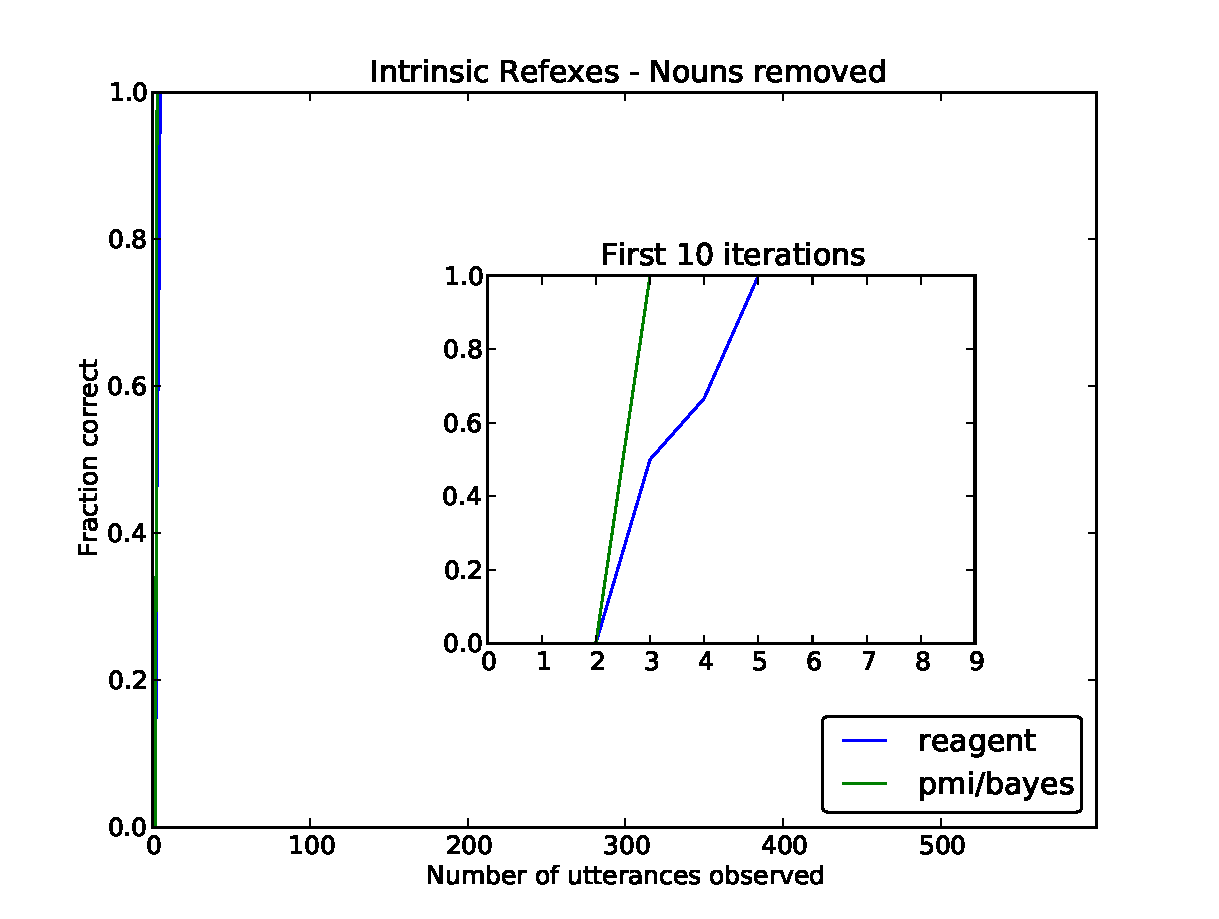
\includegraphics[scale=0.7]{grammar/1_intrinsic_refex_nouns.pdf}
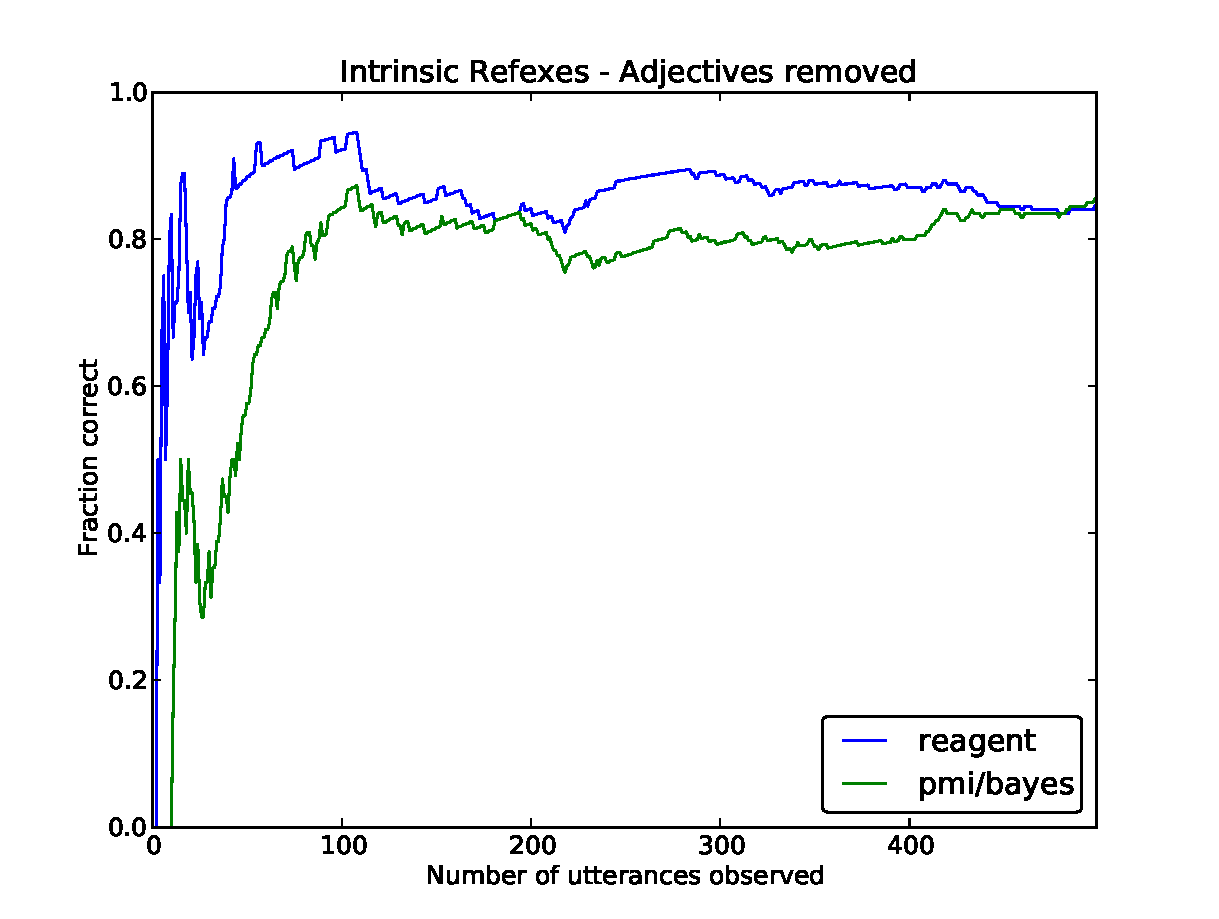
\includegraphics[scale=0.7]{grammar/2_intrinsic_refex_adjectives.pdf}
\caption{Noun and adjective learning \label{fig:adjnoun}}
\end{figure}
\newpage
\paragraph{Experiment 3 (Spatial Relations)}
The third experiment uses objects of randomly assigned colors, shapes, and locations, with utterances of the form ''The object [relation] [landmark phrase]'' and relations constructions are removed for Reagent. PMI does not perform as well here because it does not know which observations to learn from. Both methods are only told the true \textit{referent} of each utterance, but not which is the correct landmark. As feature vectors are calculated from pairs (potential referent and landmark) all pairs which have the correct referent must be considered positive examples, even though only one is truly correct. However each of these pairs does reflect that the referent is an object (and not part of the table), so PMI is able to learn that much, but then can only guess which of the 5 objects is being referred to giving it a 20\% accuracy as seen in Figure \ref{fig:relations}.
\begin{figure}[h!]
\centering
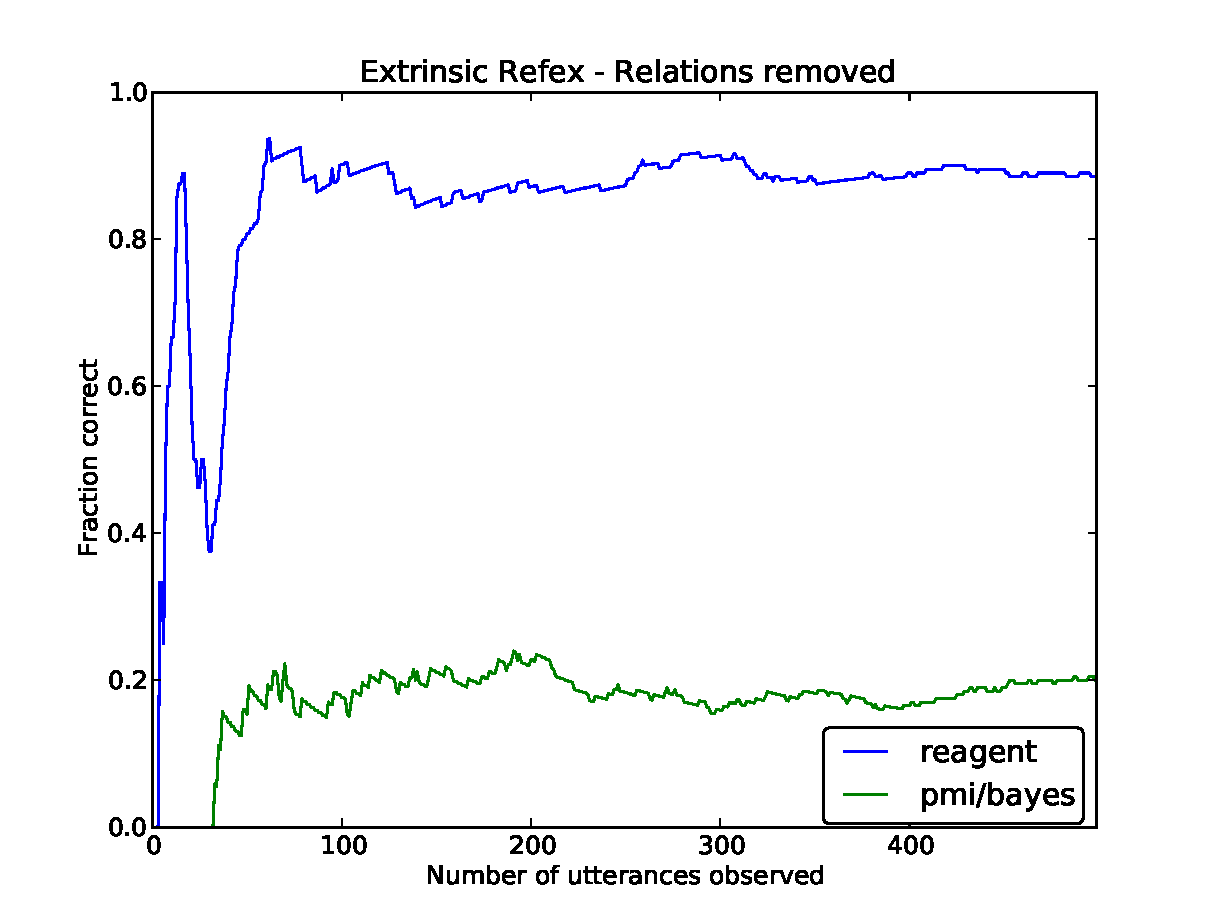
\includegraphics[scale=0.7]{grammar/3_extrinsic_refex_relations.pdf}
\caption{\label{fig:relations}}
\end{figure}
\newpage

\paragraph{Experiment 3 (Spatial Relations) - PMI Cheating}
I wanted to see if PMI would perform better with more information. I decided to let it cheat by knowing which feature vectors in its training examples used the correct landmark. However this was not enough for it to learn to interpret the landmark part of the utterance, because there were no features giving the landmark's properties in the vector. So I added in features giving the landmark's representation, color, and class for a given entity-landmark pair. With this new information PMI performs much better in Experiment 3, as seen in Figure \ref{fig:cheating}.
\begin{figure}[h!]
\centering
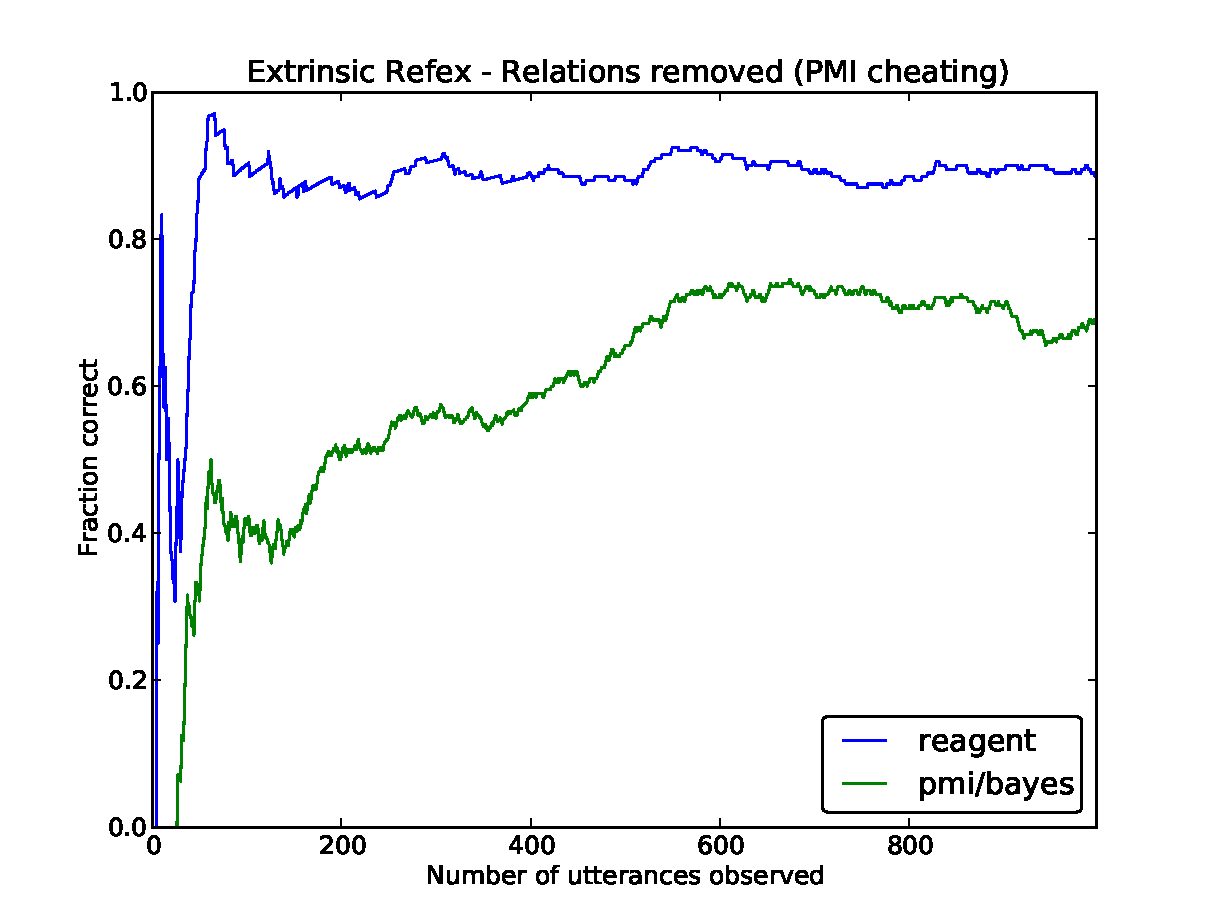
\includegraphics[scale=0.7]{grammar/4_extrinsic_refex_relations_pmi_cheating.pdf}
\caption{\label{fig:cheating}}
\end{figure}
\newpage
\paragraph{Experiment 3 (Spatial Relations) - Two-pass PMI}
In the last graph PMI had access to more information than it should, so I wanted to see if I could give it better results honestly. I removed the extra features and landmark knowledge. However, I gave the PMI baseline access to a database of intrinsic referring expressions such as those seen in Experiment 2. The baseline uses this intrinsic refex data to decide (using PMI) which landmark is most likely give all the words in the utterance. It then uses this likelihood to weight its training feature vectors according to which are most likely. It also uses this likelihood for making its decision, by giving a starting weight to each entity-landmark pair, and doing a second pass of PMI using the extrinsic refex data it is collecting in the experiment. This allows it to learn the correlation between the relation words and distance/angle/containment features, as seen in Figure \ref{fig:2pass}.

\begin{figure}[h!]
\centering
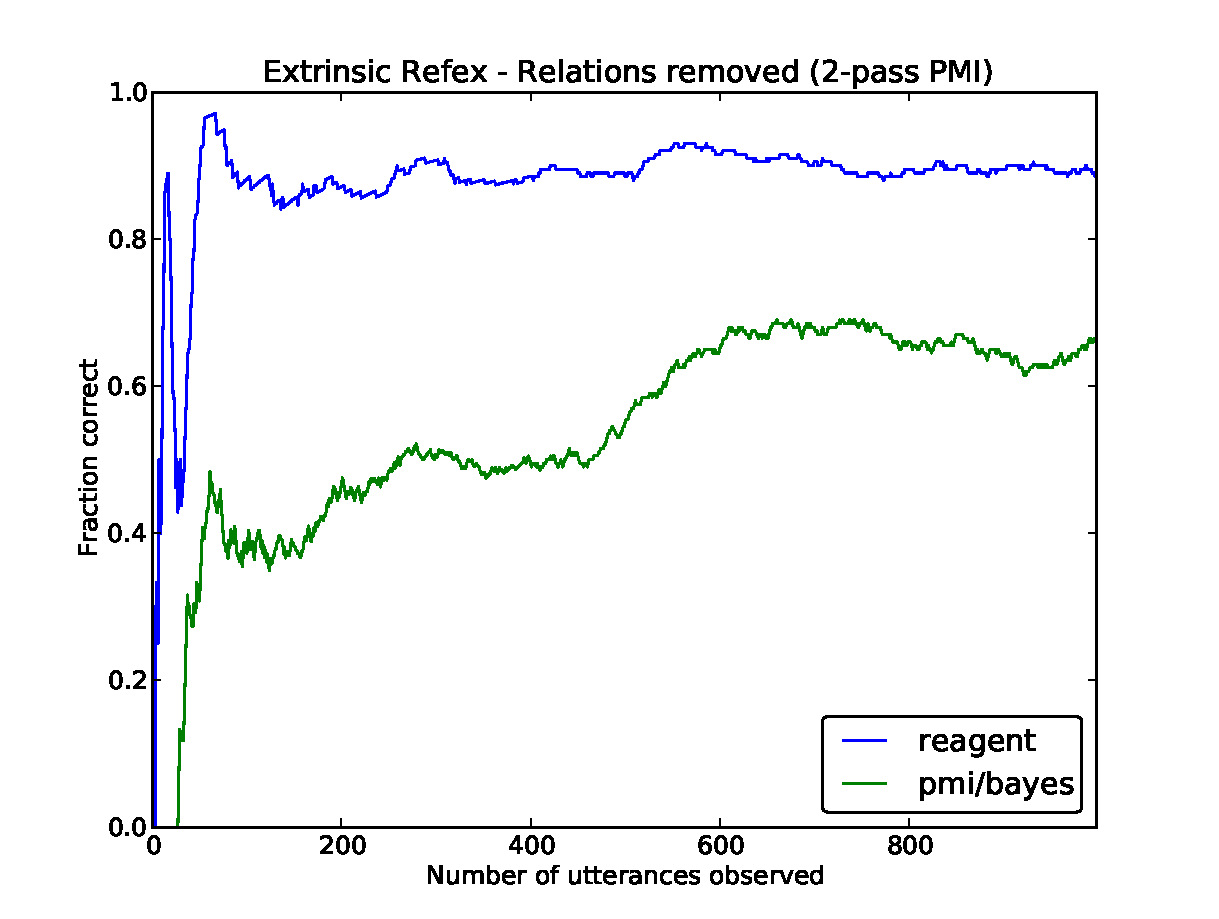
\includegraphics[scale=0.7]{grammar/5_extrinsic_refex_relations_2pass_pmi.pdf}
\caption{\label{fig:2pass}}
\end{figure}
\newpage
\paragraph{Conclusions}
Experiments 1 \& 2 show that PMI works well for this task, and Experiment 3 with cheating or two-pass PMI show that Kernel Density Estimation works for continuous features. I have no doubt that the old BOLT method which performs parsing to identify the landmark phrase could use KDE to perform equally well as Reagent at this task (but I haven't done this because it would be significant effort to get that code working alongside Reagent). 

However, Reagent has at least 2 advantages over PMI (aside from performance). First, Reagent encapsulates the special knowledge about referring expressions and landmark phrases in its constructions, so it could be used to interpret other types of utterances with only the addition of new constructions. PMI is calculated based on the knowledge that it is interpreting a referring expression or landmark phrase, so in order to interpret a different kind of expression a different PMI calculation would need to be hard-coded. The two-pass PMI also takes advantage of the specific form of Experiment 3 utterances (''The object...'') because if the utterance started ''The red cube [relation]..'' then the first (landmark) pass of PMI would get confused.

Second, PMI uses KDE for continuous features, so the representation it learns for relations is essentially a sum of gaussians. This representation of applicability functions is very accurate, but less useful than the functions Reagent learns. For instance, for ''near to'' Reagent learns a sigmoid AF, and in the future Reagent could learn that ''very'' can modify ''near to'' by pushing the sigmoid's inflection point towards 0. PMI on the other hand would have to learn a separate KDE estimate for ''very near to'' and has no way of generalizing between the two applicability functions.






\end{document}